\subsection*{Task 3}

\subsubsection*{a)}

\subsubsection*{Network 1}

The first network is almost identical with the one in Task 2, and has the architecture shown in \cref{tab:task3:net1}. The convolutional layers use $5\times5$ filters, with a stride of 1 and a padding of 2, while the pooling layers use a stride of 2 and kernel size of $2\times2$. The batch size is 64, and the network uses early stopping. The network uses a SGD optimizer, with no regularization, data augmentation or weight initialization (other than PyTorch's default Kaiming initialization). The learning rate is initially set to 0.05, but the network uses a learning rate scheduler that decreases the learning rate by 0.1 every fourth epoch. 

\begin{table}[h!]
    \centering
    \begin{tabular}{|c|c|c|c|}
      \hline
      Layer & Layer Type & Hidden Units/Filters & Activation \\
      \hline
      1 & Conv2D & 32 & ReLU \\
      1 & BatchNorm2D & - & - \\
      1 & MaxPool2D & - & - \\
      \hline
      2 & Conv2D & 64 & ReLU \\
      2 & BatchNorm2D & - & - \\
      2 & MaxPool2D & - & - \\
      \hline
      3 & Conv2D & 128 & ReLU \\
      3 & BatchNorm2D & - & - \\
      3 & MaxPool2D & - & - \\
      \hline
        & Flatten & - & - \\
      \hline
      4 & Dense & 64 & ReLU \\
      4 & BatchNorm1D & - & - \\
      \hline
      5 & Dense & 10 & ReLU \\
      \hline
    \end{tabular}
    \caption{Network 1 architecture.}
    \label{tab:task3:net1}
\end{table}


\subsubsection*{Network 2}

\begin{table}[h!]
    \centering
    \begin{tabular}{|c|c|c|c|}
      \hline
      Layer & Layer Type & Hidden Units/Filters & Activation \\
      \hline
      1 & Conv2D & 32 & ReLU \\
      1 & BatchNorm2D & - & - \\
      1 & Conv2D & 32 & ReLU \\
      1 & BatchNorm2D & - & - \\
      1 & MaxPool2D & - & - \\
      \hline
      2 & Conv2D & 64 & ReLU \\
      2 & BatchNorm2D & - & - \\
      2 & Conv2D & 64 & ReLU \\
      2 & BatchNorm2D & - & - \\
      2 & MaxPool2D & - & - \\
      \hline
      3 & Conv2D & 128 & ReLU \\
      3 & BatchNorm2D & - & - \\
      3 & Conv2D & 128 & ReLU \\
      3 & BatchNorm2D & - & - \\
      3 & MaxPool2D & - & - \\
      \hline
        & Flatten & - & - \\
      \hline
      4 & Dense & 64 & ReLU \\
      4 & BatchNorm1D & - & - \\
      \hline
      5 & Dense & 10 & ReLU \\
      \hline
    \end{tabular}
    \caption{Network 2 architecture.}
    \label{tab:task3:net2}
\end{table}

The second network has architecture shown in \cref{tab:task3:net2}. The convolutional layers use identical filters to Network 1, in addition to identical max-pooling. The batch size is 64 here as well. Early stopping is turned off here (as this gave a slight increase in accuracy), and no regularization, data augmentation or weight initialization is used here either, and it uses a SGD optimizer. The learning rate is here set to 0.1, and decreases by 0.25 every fourth epoch.


\subsubsection*{b)}

\begin{table}[h!]
  \centering
  \begin{tabular}{|l|c|c|}
    \hline
    Metric & Network 1 & Network 2 \\
    \hline
    Training loss & 0.2460 & 0.1484 \\
    Training accuracy & 0.9297 & 0.9590 \\
    Validation accuracy & 0.7528 & 0.8111 \\
    Test accuracy & 0.7659 & 0.8193 \\
    \hline
  \end{tabular}
  \caption{Performance metrics of the two networks.}
  \label{tab:task3:performance}
\end{table}

\begin{figure}[h!]
  \centering
  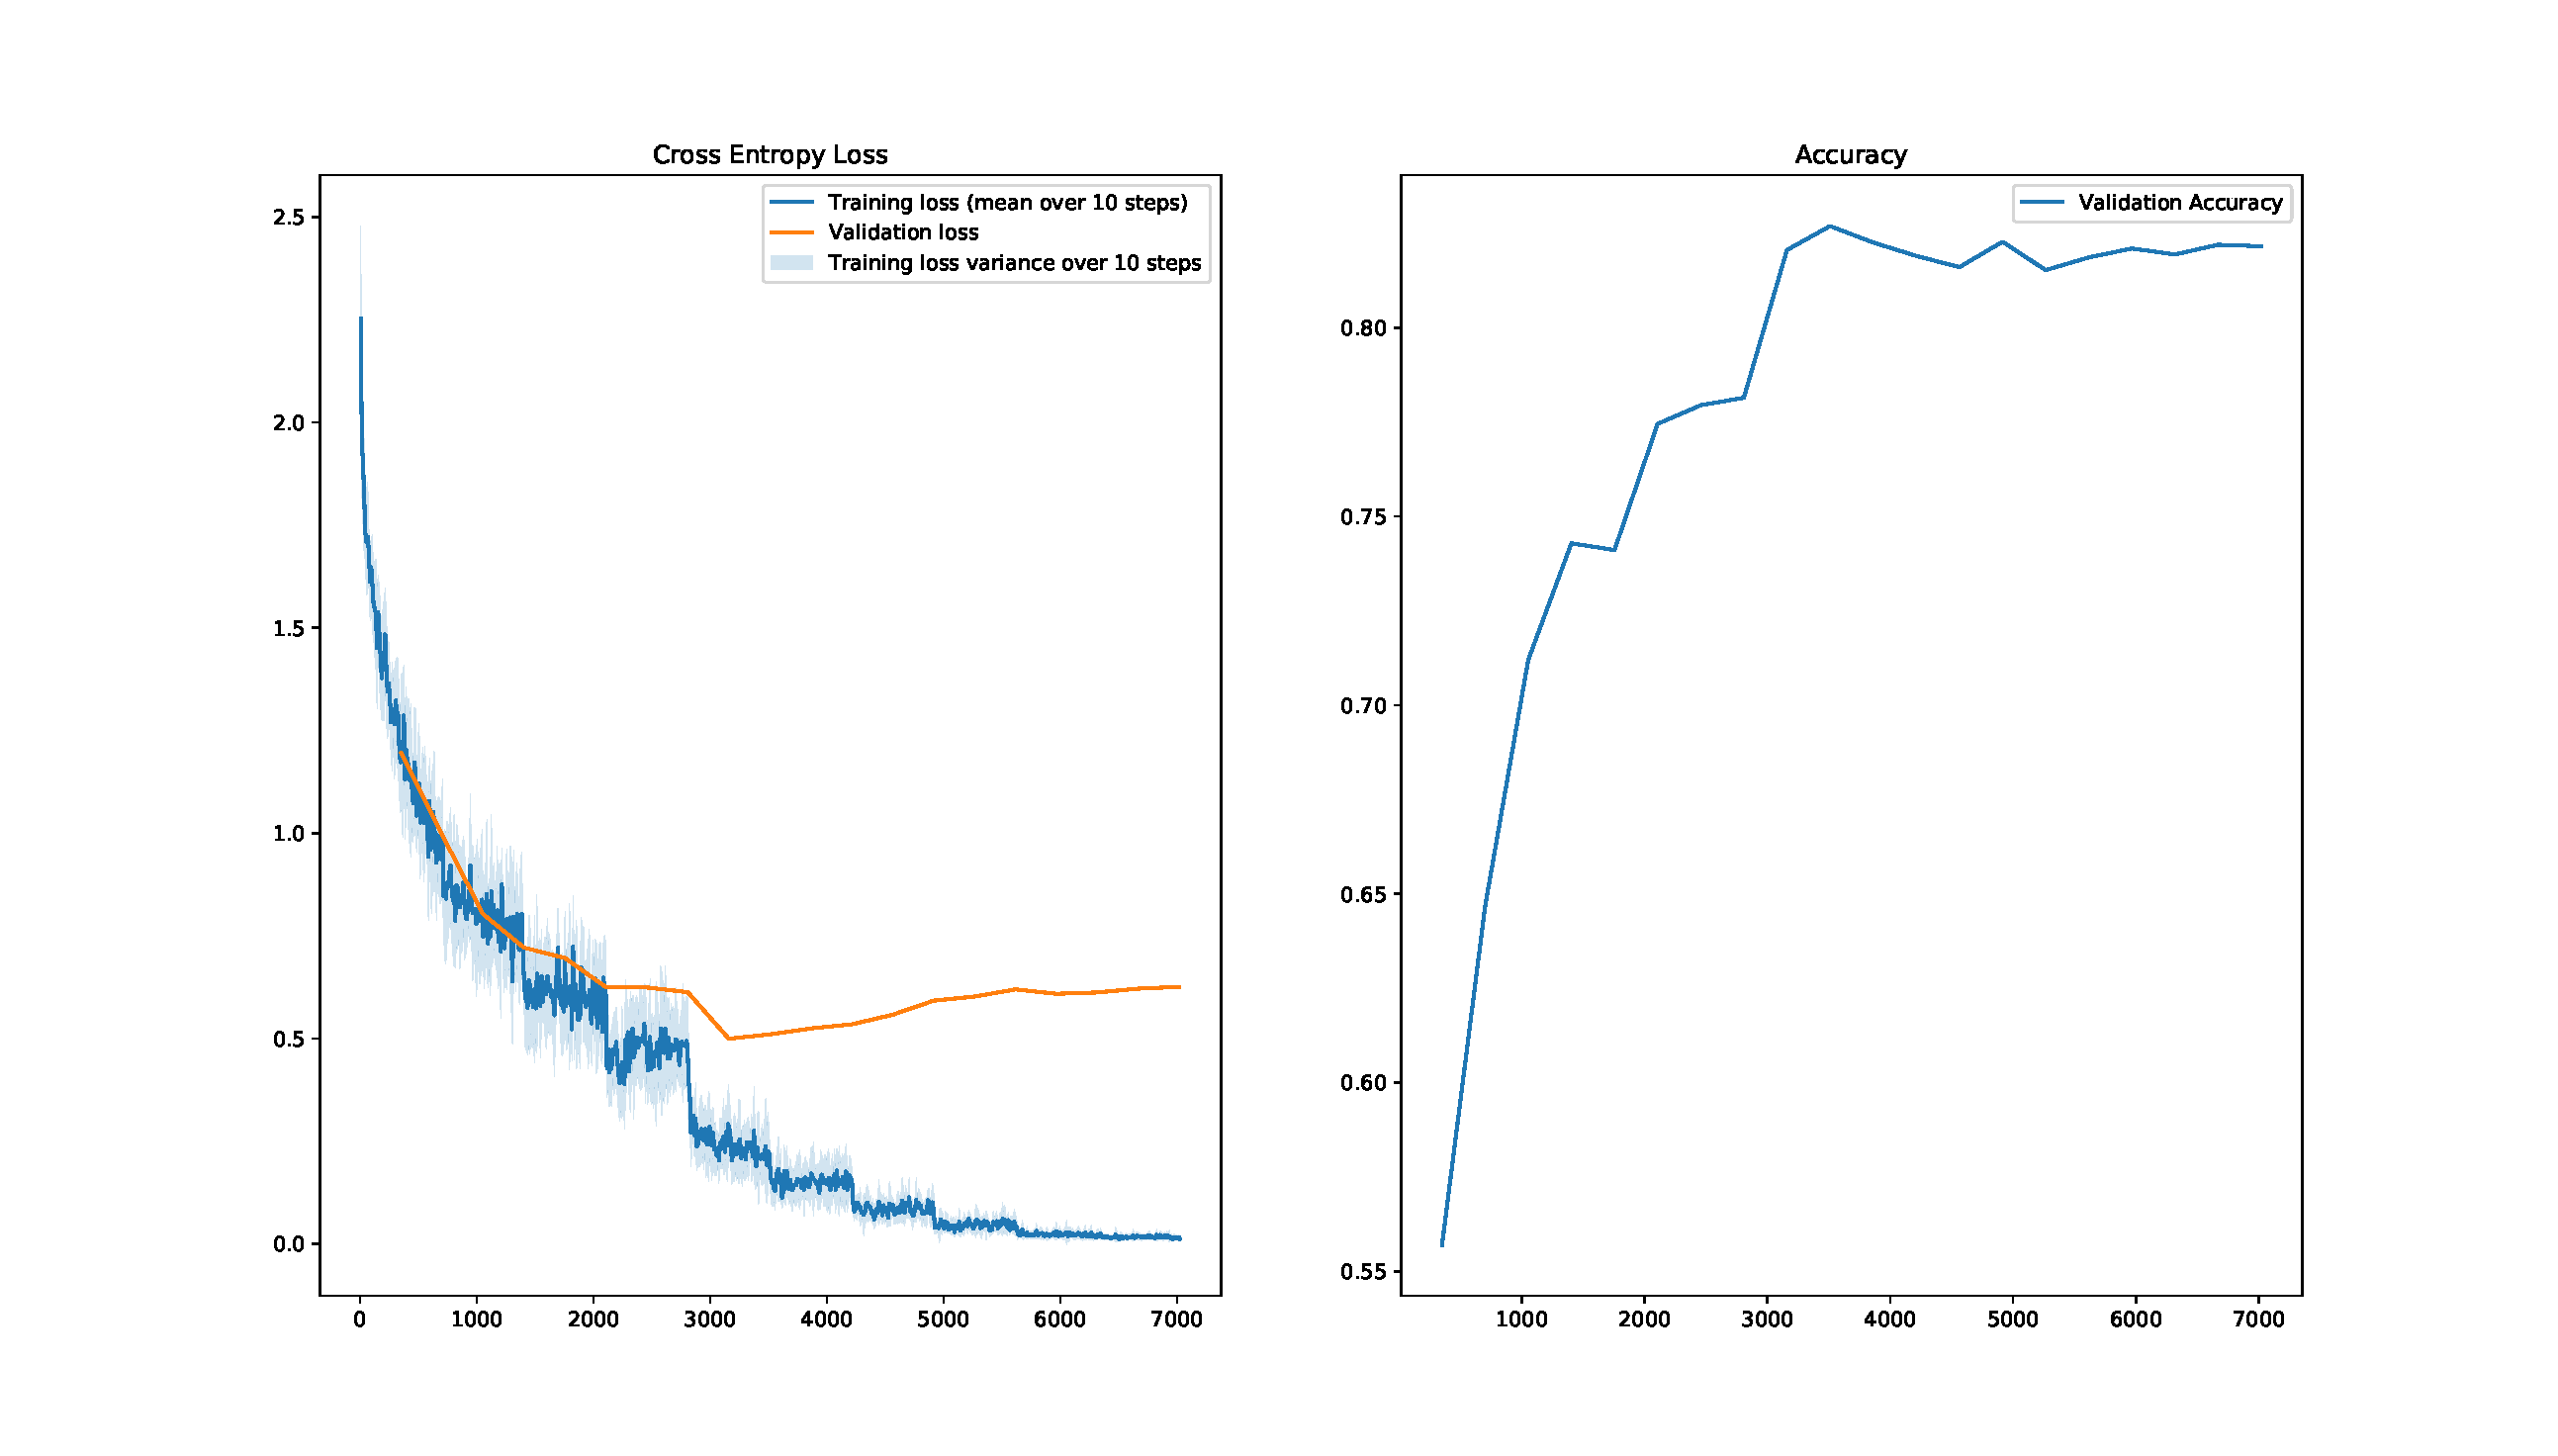
\includegraphics[clip, trim = 3cm 0cm 3cm 0cm, width=\textwidth]{figures/Task3b.pdf}
  \caption{Training and validation loss (left) and validation accuracy (right) over training for Network 2.}
  \label{fig:task3:b}
\end{figure}


\subsubsection*{c)}

I used the model from Task 2 as baseline, and iteratively changed parameters and architecture. I found that surprisingly many parameters where good as they were, and that by introducing e.g data augmentation and different weight initialization, optimizer and activation functions, the performance only worsened. However, batch normalization and learning rate scheduling improved the performance by a large margin.

The implementation of data augmentation is probably poor, as it augments both the training and validation set, which may result in poorer performance on the test set. I found that the training set was large enough as it was, and did therefore not feel the need to spend more time on data augmentation.

Different weight initialization methods worked fined, but none gave better performance than the default Kaiming initialization. This apparently works well with ReLU, and keeps the variance around 1, so we avoid exploding or vanishing gradients. This also applies to e.g Xavier and normal initialization, so I am not exactly sure why Kaiming performs better.

I tried different activation functions, where ReLU, ELU and LeakyReLU performed similarly. Using sigmoid or tanh did not work well, as the network converged very slowly with these. 

The Adam optimizer was tried out instead of SGD, but gave poor numerical stability. This may only be a matter of tuning the $\beta$-values in the optimizer, which would probably fix the issues, but I stuck with SGD as it seemed to work fine. Adam had a slightly faster convergence, so better tuning might give better performance than SGD.

The original filters and pooling layers from Task 2 performed best as well. A smaller filter size on the convolutional layer also worked fine, but larger filters did not perform as well. The reason for this may be that a too large size will not capture the features of the image precisely, making it difficult to learn the specific features of a class. Using strided convolutions instead of pooling did not work either, perhaps because this introduces more parameters in the network.

Batch normalization gave the largest improvement in performance, and was used after each convolution. This increased the convergence speed dramatically, and allowed for a higher learning rate, which in combination with a learning rate scheduler gave best performance. The learning rate was large in the first epochs, giving fast convergence, and was lowered later on as the network converged to a minima.

\subsubsection*{d)}

\begin{figure}[h!]
  \centering
  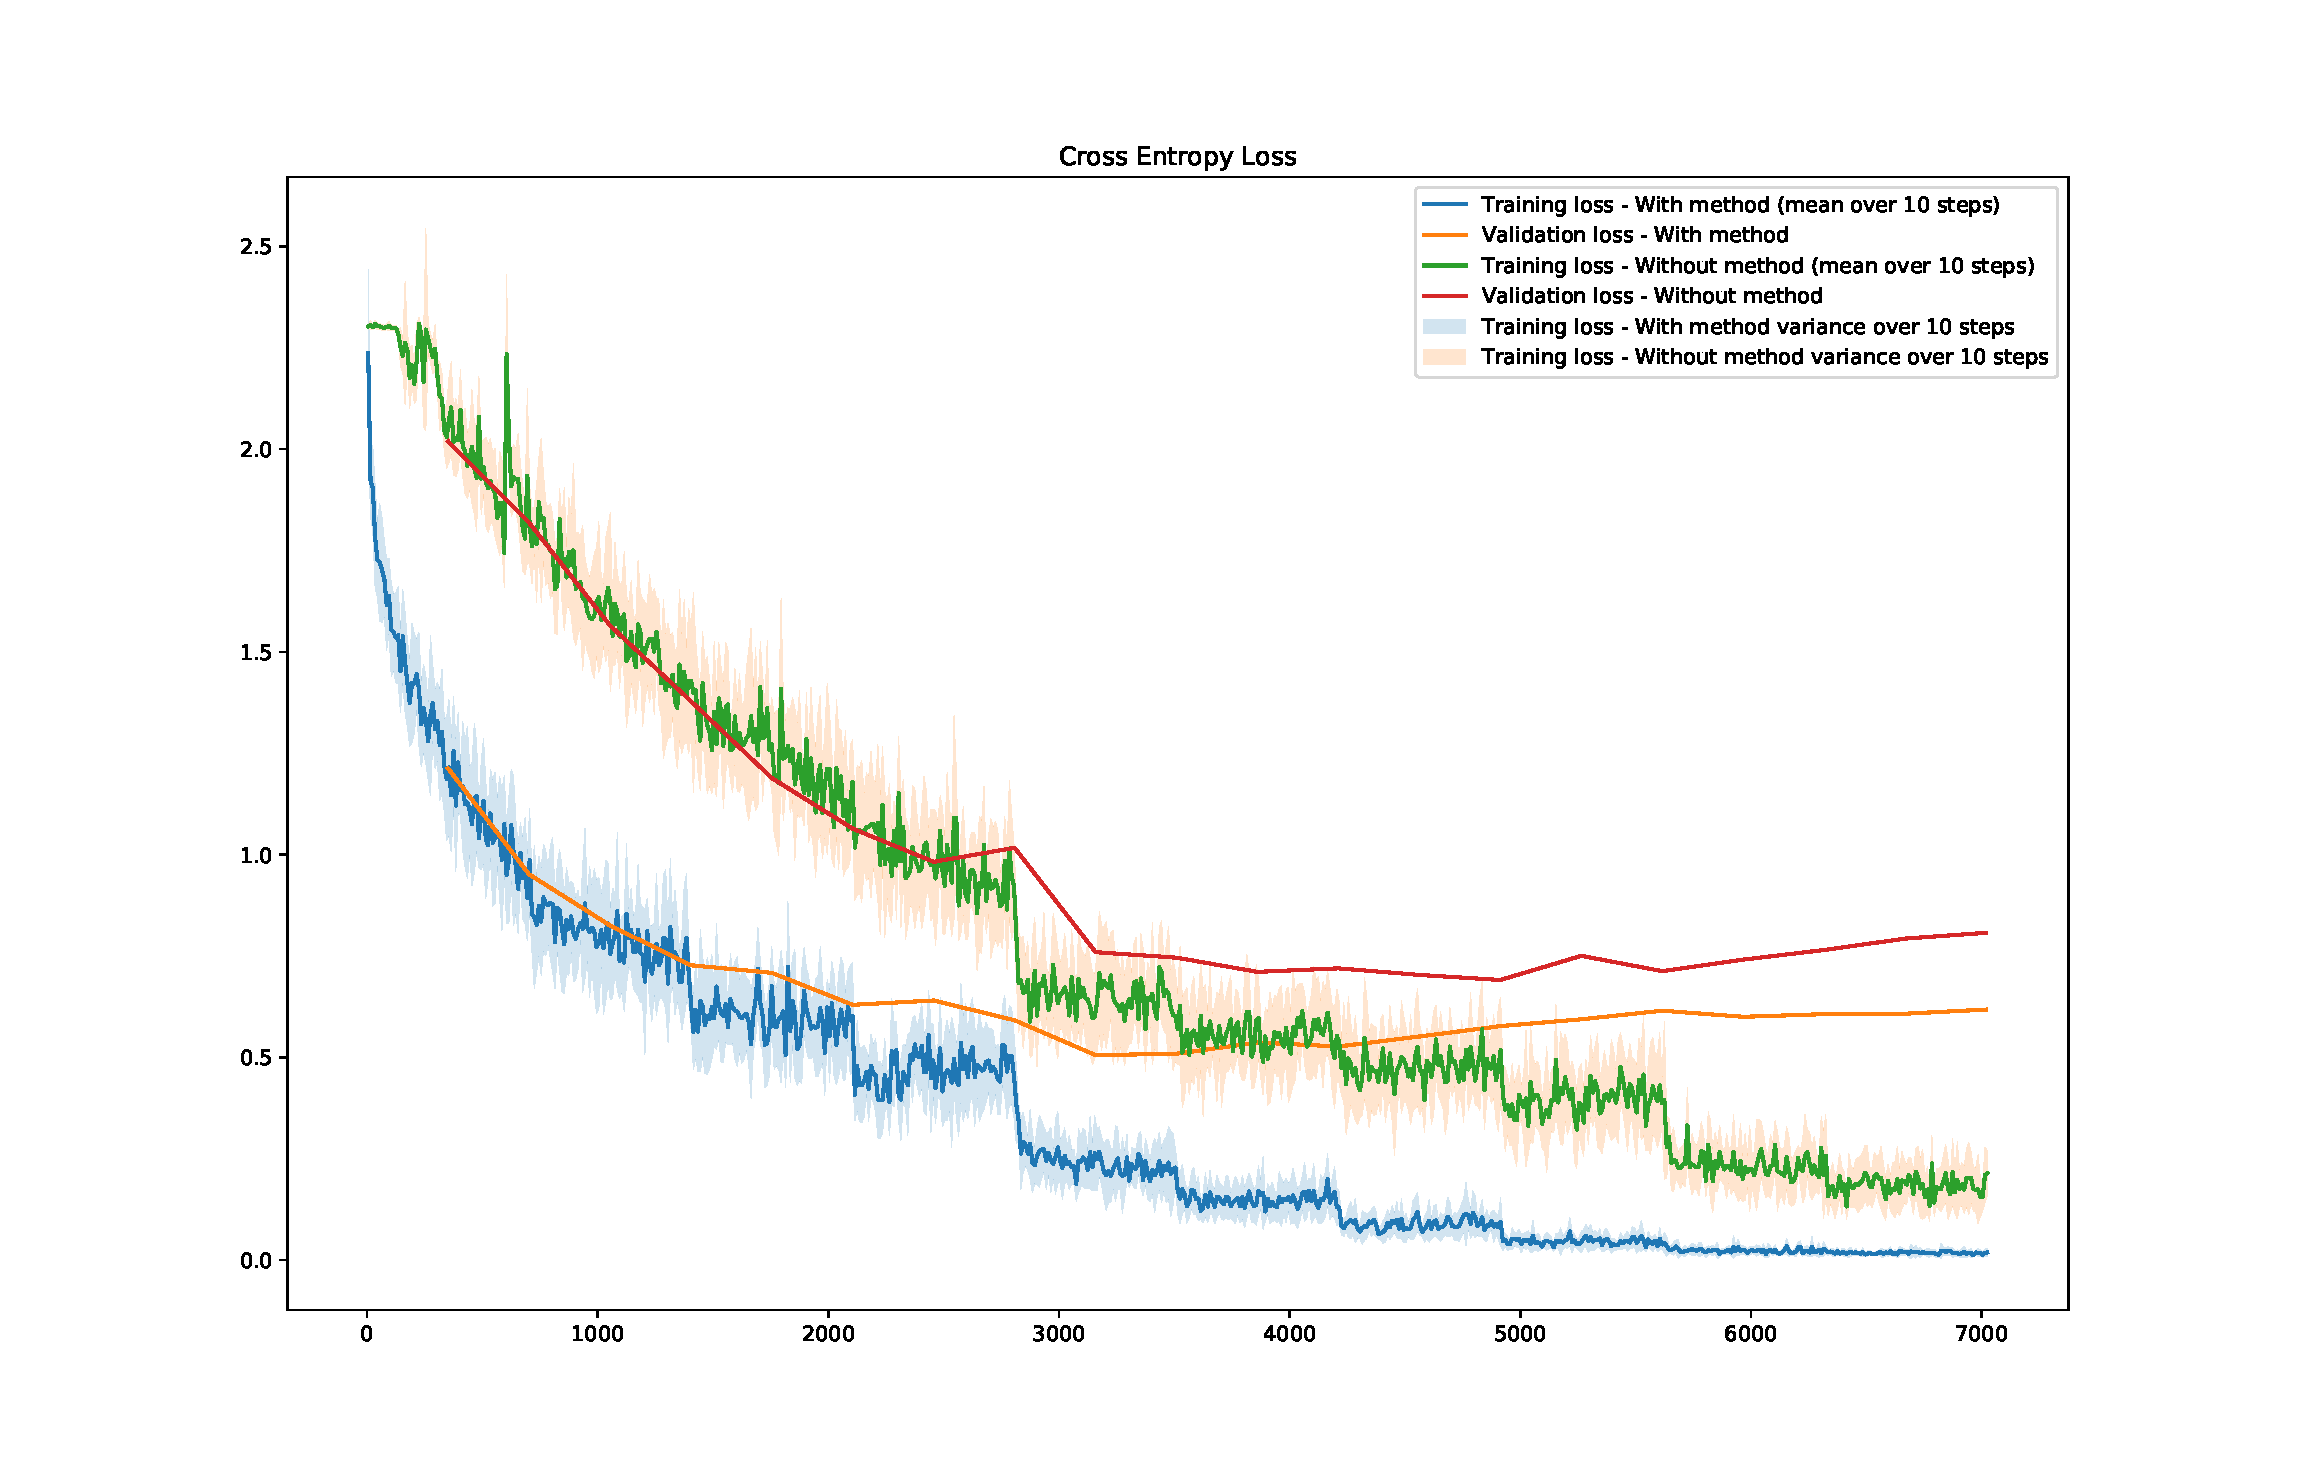
\includegraphics[clip, trim = 0cm 0cm 0cm 0cm, width=\textwidth]{figures/Task3d-batch.pdf}
  \caption{Comparison of training and validation loss with and without batch normalization.}
  \label{fig:task3:d}
\end{figure}


\subsubsection*{e)}

Network 2 has an accuracy slightly above 80\%, as shown in \cref{tab:task3:performance}, with validation accuracy shown in \cref{fig:task3:b}.


\subsubsection*{f)}

In \cref{fig:task3:b} we see clear signs of overfitting, as the validation loss stalls while the training loss continues to decrease. This was remedied by using both dropout and $L_2$-regularization, but at the cost of a decrease in test accuracy below 80\%, so this was not used in the final network. One could perhaps argue that as long as the test accuracy is high, the model is sufficiently generalized. This could however only be that the given test set fits well with the trained model, but other data may not. If given more time, I would therefore try to find a model that achieves above 80\% accuracy while also using regularization. 
